% This file is generated by the MATLAB m-file laprint.m. It can be included
% into LaTeX documents using the packages graphicx, color and psfrag.
% It is accompanied by a postscript file. A sample LaTeX file is:
%    \documentclass{article}\usepackage{graphicx,color,psfrag}
%    \begin{document}\input{Loglin_E}\end{document}
% See http://www.mathworks.de/matlabcentral/fileexchange/loadFile.do?objectId=4638
% for recent versions of laprint.m.
%
% created by:           LaPrint version 3.16 (13.9.2004)
% created on:           01-Jul-2011 12:37:53
% eps bounding box:     15 cm x 11.25 cm
% comment:              
%
\begin{psfrags}%
\psfragscanon%
%
% text strings:
\psfrag{s03}[t][t]{\color[rgb]{0,0,0}\setlength{\tabcolsep}{0pt}\begin{tabular}{c}{\Large$f/\mathrm{Hz}$}\end{tabular}}%
\psfrag{s04}[b][b]{\color[rgb]{0,0,0}\setlength{\tabcolsep}{0pt}\begin{tabular}{c}{\Large$(\mathrm{d}E/\mathrm{d}{f})/\left(10^{42} \times \mathrm{J\,Hz}^{-1}\right)$}\end{tabular}}%
%
% xticklabels:
\psfrag{x01}[t][t]{$10^{-6}$}%
\psfrag{x02}[t][t]{$10^{-5}$}%
\psfrag{x03}[t][t]{$10^{-4}$}%
\psfrag{x04}[t][t]{$10^{-3}$}%
\psfrag{x05}[t][t]{$10^{-2}$}%
\psfrag{x06}[t][t]{$10^{-1}$}%
%
% yticklabels:
\psfrag{v01}[r][r]{$0.0$}%
\psfrag{v02}[r][r]{$0.5$}%
\psfrag{v03}[r][r]{$1.0$}%
\psfrag{v04}[r][r]{$1.5$}%
\psfrag{v05}[r][r]{$2.0$}%
\psfrag{v06}[r][r]{$2.5$}%
\psfrag{v07}[r][r]{$3.0$}%
\psfrag{v08}[r][r]{$3.5$}%
\psfrag{v09}[r][r]{$4.0$}%
\psfrag{v10}[r][r]{$4.5$}%
\psfrag{v11}[r][r]{$5.0$}%
%
% Figure:
\resizebox{12cm}{!}{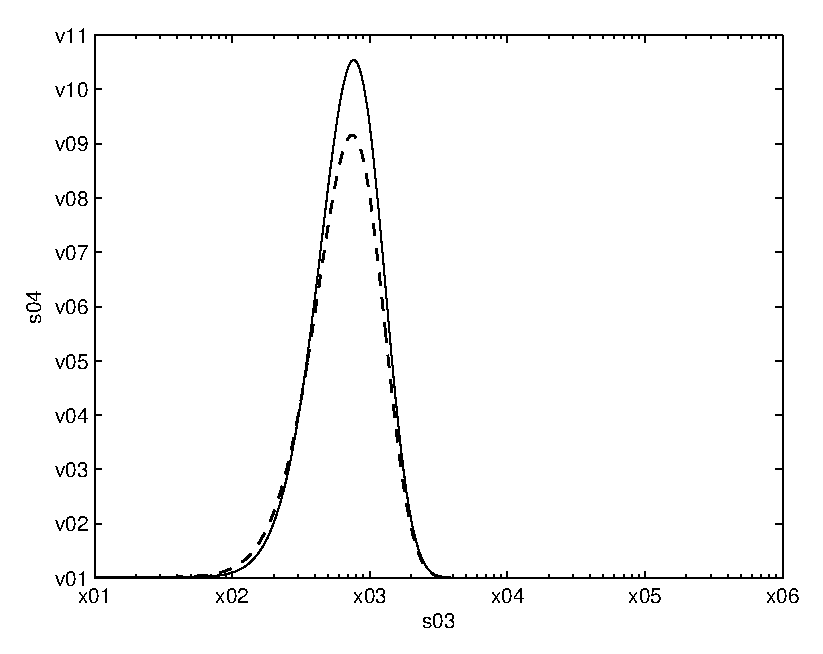
\includegraphics{Loglin_E_30.eps}}%
\end{psfrags}%
%
% End Loglin_E.tex
% E_quad = 4.769858090725944e+38
% E_oct = 5.077439176908533e+38
% E_PM = 4.411756497228369e+38
